\documentclass[tikz,convert={outext=.svg,command=\unexpanded{pdf2svg \infile\space\outfile}},multi=false]{standalone}
\usepackage[utf8]{inputenc}

\usetikzlibrary{automata}% tikz package already loaded by 'tikz' option
\begin{document}

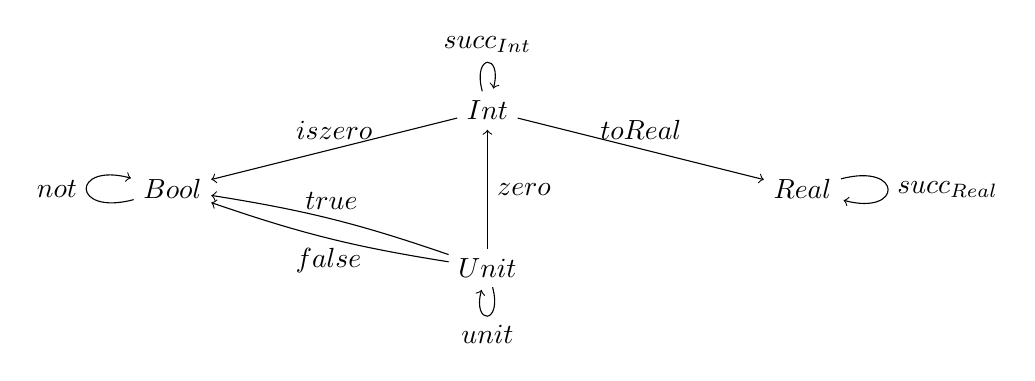
\begin{tikzpicture}[xscale=1]
\node (Bool) {$Bool$};
\node (Int) at (4, 1) {$Int$};
\node (Real) at (8, 0) {$Real$};
\node (Unit) at (4, -1) {$Unit$};
\draw[->] (Bool) edge[loop left] node[left] {$not$} (Bool);
\draw[->] (Int) edge[loop above] node[above] {$succ_{Int}$} (Int);
\draw[->] (Real) edge[loop right] node[right] {$succ_{Real}$} (Real);
\draw[->] (Unit) edge[loop below] node[below] {$unit$} (Unit);
\draw[->] (Int) edge node[above] {$iszero$} (Bool);
\draw[->] (Int) edge node[above] {$toReal$} (Real);
\draw[->] (Unit) edge node[right] {$zero$} (Int);
\draw[->] (Unit) edge[bend right=5] node[above] {$true$} (Bool);
\draw[->] (Unit) edge[bend left=5] node[below] {$false$} (Bool);
\end{tikzpicture}
\end{document}